% The first argument is the \documentclass, which tells latex which template
% we're using to build this document. It's usually safe to just use "article".
\documentclass{article}

% include some packages...
\usepackage{fullpage} % change settings for a smaller margin
\usepackage{graphicx} % gives access to the \includegraphics commands
\usepackage{amsfonts}
\usepackage{float}
\usepackage{enumitem}
\usepackage{caption}
\usepackage[export]{adjustbox}
\usepackage{bookmark}
% \usepackage{subfiles}
\graphicspath{{./images/}}

% tell Latex to use no paragraph indentation, but leave some space between
% paragraphs
\setlength{\parindent}{0in}
\setlength{\parskip}{0.1in}

\newcommand{\tib}[1]{\textit{\textbf{#1}}}
\newcommand{\code}[1]{\texttt{#1}}

% Remove blank pages
%\let\cleardoublepage=\clearpage

% these commands merely set the values for the title/date/author; they don't put
% them in the document... see \maketitle below
\title{CS Department Automated Information Timeline \\ Iteration 1 Submission}
\date{February 5, 2024}
\author{Matthew Hays, Pawan Bhandari, Sarah Faron, Tim Klimpel}

% all document content goes between \begin{document} and \end{document}
\begin{document}

% this command actually creates the title/date/author in the document
\maketitle
\newpage
\tableofcontents
\listoffigures
\newpage
%%%%%%%%%%%%%%%%%%%%%%%%%%%%%%%%%%%%%%%%%%%%%%%%%%%%%%%%%%%%%%%%%%%%%%%%%%%%%%%
\section{Vision Statement}

The Baylor University Computer Science Department needs a system for faculty to passively share information on department news and events with students and other faculty members. To fulfill this need, our team is developing an automated, web-based system that will populate faculty content, perform content rolling, and automate content updates. \\

Using our system, any faculty can propose a post, but only one admin/reviewer can approve the post for publishing. In addition to the embedded post timeline, the system also has an event calendar. Similarly, any faculty can propose an event to add to the calendar, but only one admin/reviewer can approve the event for publishing to the event calendar. \\

This content is available for viewing through a TV screen in the department lobby, which is manually managed by our CS Department office manager. The system is configured to either (1) show only the most recent content on the lobby TV or (2) show staged media tagged manually by the office manager. The system uses \hyperref[sec:Glossary]{WebSockets} to roll and update recent content automatically, as well as a \hyperref[sec:Glossary]{WYSIWYG} editor to modify and tag static content pages. \\

Since not everything can be displayed in the lobby, the system suppports a web view accessible to all visitors with a mobile device via QR code. Through the web application, all audience members can browse all content available beyond the posts and events tagged for the lobby TV. \\

The system uses Spring middleware with database and REST API to support the two described web-based and UI-responsive frontends. \\
%%%%%%%%%%%%%%%%%%%%%%%%%%%%%%%%%%%%%%%%%%%%%%%%%%%%%%%%%%%%%%%%%%%%%%%%%%%%%%%
\section{Requirements}
\subsection{Functional Requirements}

\textbf{REQ01:} Faculty members can create a post for review, which will initially default to a proposed state until approved. \\
\textbf{REQ02:} An admin/reviewer must approve a post before it can be published to the site. \\
\textbf{REQ03:} A user can add events to an event calendar that can be displayed on screen. \\
\textbf{REQ04:} A user can add pictures to posts. \\
\textbf{REQ05:} A user can add videos to posts. \\
\textbf{REQ06:} A user can add HTML pages to posts. \\
\textbf{REQ07:} A user can tag approved posts for display on a large format screen. \\
\textbf{REQ08:} The system will allow management of which posts are displayed. \\
\textbf{REQ09:} The system will allow management of which media is displayed. \\
\textbf{REQ10:} The system will fall back to the 10 most recent posts if no posts are tagged, or less than 10 posts are tagged. \\
\textbf{REQ11:} The Office manager will use the WYSIWYG editor to modify static content posts. \\
\textbf{REQ12:} The Office Manager will use the WYSIWYG editor to tag posts for display on screen. \\
\textbf{REQ13:} The system will allow audiences to use their mobile devices (e.g., through a QR code that brings them to the website) to browse all content beyond the 10 most recent posts. \\
\textbf{REQ14:} The system will allow audiences to use their mobile device to browse the calendar. \\
\textbf{REQ15:} A user will authenticate and be assigned a valid role or view the content as a non-authenticated user. \\
%%%%%%%%%%%%%%%%%%%%%%%%%%%%%%%%%%%%%%%%%%%%%%%%%%%%%%%%%%%%%%%%%%%%%%%%%%%%%%%
\subsection{Non-Functional Requirements}

\textbf{REQ16:} The system will have the following user roles: Faculty, Admin, and Office Manager. \\
\textbf{REQ17:} Content rolling and updates to content will be completed via WebSockets. \\
\textbf{REQ18:} The backend will consist of a Spring Framework REST API with a database and appropriate middleware. \\
\textbf{REQ19:} The system will manage a media library which consists of all posted pictures and videos. \\
\textbf{REQ20:} The system will consist of a front-end display: a television screen. \\
\textbf{REQ21:} The system will consist of a front-end display: a web-based display optimized for all screen sizes. \\
\textbf{REQ22:} The design of the user interface must utilize Baylor's official \href{https://brand.web.baylor.edu/brand-standards/official-brand-colors}{color scheme}.
\begin{itemize}
    \item Baylor Green: \#154734
    \item University Gold: \#FFB81C
    \item Secondary and accent colors can be chosen from the lists provided \href{https://brand.web.baylor.edu/brand-guidelines/design-colors}{here}.
\end{itemize}
\textbf{REQ23:} The system will have a WYSIWYG editor.
%%%%%%%%%%%%%%%%%%%%%%%%%%%%%%%%%%%%%%%%%%%%%%%%%%%%%%%%%%%%%%%%%%%%%%%%%%%%%%%
\section{Glossary} \label{sec:Glossary}

The following terms are important to the development of the project:
\begin{itemize}
    \item \textbf{WYSIWYG Editor:} What You See Is What You Get editor
    \item \textbf{WebSocket:}
    \item \textbf{Post:} A picture, video, or manually created html page.
    \item \textbf{Page:}
    \item \textbf{Event Calendar:} A calendar which is displayed on screen which faculty can add events.
    \item \textbf{Media Library:} A library which stores both picture and video content.
    \item \textbf{Faculty:} Admin, Reviewer, Officer Manager, and other university employee.
    \item \textbf{Admin:} A privileged user that holds all access rights.
    \item \textbf{Reviewer:} A user that acts as a reviewer of posts to approve or reject posts that have been submitted for review.
    \item \textbf{Officer Manager:} A faculty member that holds special privilege over the system under discussion to manage which posts are displayed at any given time.
\end{itemize}
%%%%%%%%%%%%%%%%%%%%%%%%%%%%%%%%%%%%%%%%%%%%%%%%%%%%%%%%%%%%%%%%%%%%%%%%%%%%%%%
\section{Domain Model}

The below Domain model represents a Draft version of the current planned domain model.  Classes/objects are noted with a \textit{\_D} to indicate they are \textit{draft} classes.

\begin{figure}[H]
    \centering
    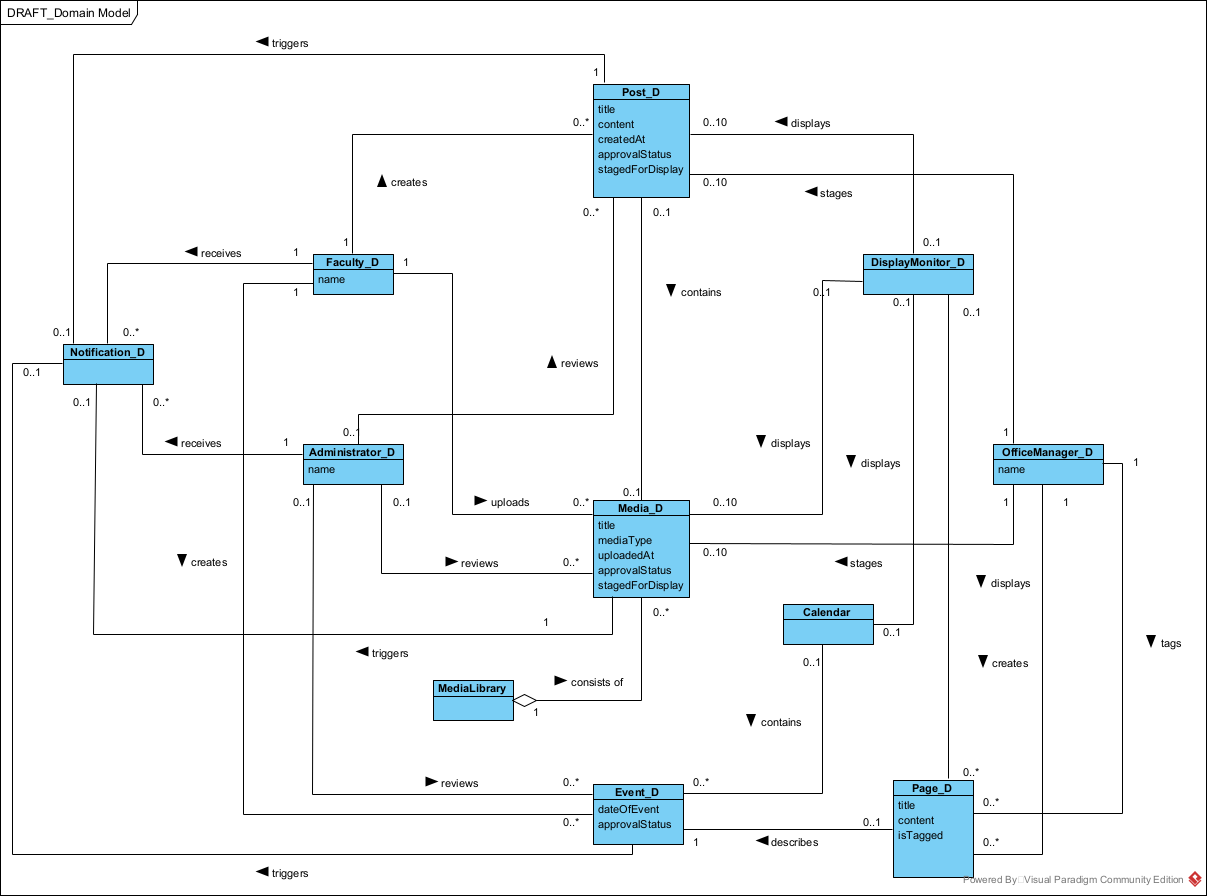
\includegraphics[width=0.8\textwidth]{images/DomainModel.png}
    \centering
    \caption{Domain Model for CS Department Automated Information Timeline}
\end{figure}
%%%%%%%%%%%%%%%%%%%%%%%%%%%%%%%%%%%%%%%%%%%%%%%%%%%%%%%%%%%%%%%%%%%%%%%%%%%%%%%
\section{Use Cases}
\subsection{Use Case Diagram}
\begin{figure}[H]
    \centering
    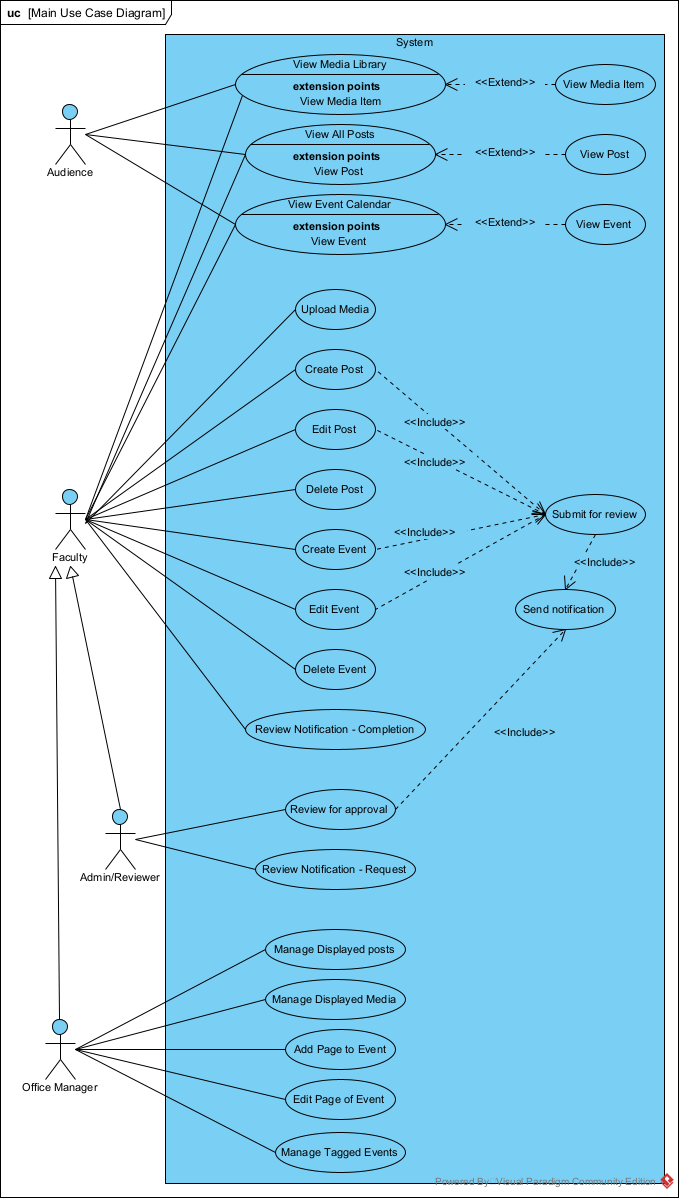
\includegraphics[width=0.64\textwidth]{images/UCD.png}
    \centering
    \caption{Use Case Diagram for CS Department Automated Information Timeline}
\end{figure}
%%%%%%%%%%%%%%%%%%%%%%%%%%%%%%%%%%%%%%%%%%%%%%%%%%%%%%%%%%%%%%%%%%%%%%%%%%%%%%%
\subsection{Use Cases}
There are a total of 16 use cases written at this stage in the project. Each team member was assigned 3 use cases to fully analyze. Each of these 12 use cases are written in fully-dressed form and accompanied by System Sequence Diagrams (SSDs) and Operations Contracts (OCs). The remaining 4 use cases are written in brief/casual form.

The assigned (fully-dressed) use cases are as follows:

\begin{center}
    \begin{tabular}{ | c | c | c | c | }
        \hline
        Bhandari & Faron & Hays & Klimpel \\
        \hline
        UC11     & UC05  & UC04 & UC15    \\
        \hline
        UC12     & UC06  & UC09 & UC16    \\
        \hline
        UC13     & UC07  & UC10 & UC01    \\
        \hline
    \end{tabular}
\end{center}
%%%%%%%%%%%%%%%%%%%%%%%%%%%%%%%%%%%%%%%%%%%%%%%%%%%%%%%%%%%%%%%%%%%%%%%%%%%%%%%
\subsubsection{UC01: View Media Library}
\textbf{ID:} UC01 (View Media Library) \\
\textbf{Scope:} CS Automated Information Timeline \\
\textbf{Level:} User goal \\
\textbf{Primary Actor:} Audience \\
\textbf{Stakeholders and Interests:}
\begin{itemize}
    \item Audience wants the ability to view all shared media through the media library
    \item Faculty wants to be able to allow guests to view media shared by them
    \item Office Manager wants to ensure that all media is available to be seen through the web portal
    \item Admin wants to be sure that approved media can be displayed to the audience
\end{itemize}
\textbf{Preconditions:}
\begin{itemize}
    \item Media library contains approved media items
\end{itemize}
\textbf{Postconditions:}
\begin{itemize}
    \item Media library is shared with the audience
\end{itemize}
\textbf{Main Success Scenario:}
\begin{enumerate}
    \item Audience member scans available QR code
    \item System provides appropriate URL for main home page
    \item Audience member navigates to URL
    \item Audience member selects “Media library” option
    \item System presents full media library view
\end{enumerate}
\textbf{Alternative Flows:} \\
3A: URL is down
\begin{enumerate}
    \item Audience member alerts faculty or office manager
    \item Office manager or faculty review system status
\end{enumerate}
5A: Multiple pages available
\begin{enumerate}
    \item System presents paged view with limit of items
    \item Audience member selects `next page'
    \item System returns next set of results
    \item Continue until end of media library is returned
\end{enumerate}

\begin{figure}[H]
    \centering
    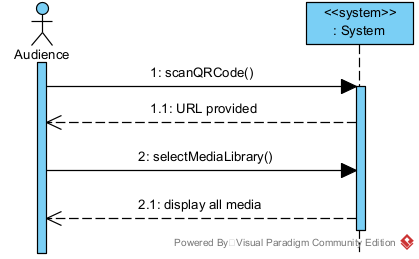
\includegraphics[width=0.8\textwidth]{images/SSD-UC01-ViewMediaLibrary.png}
    \centering
    \caption{System Sequence Diagram: View Media Library}
\end{figure}

\textbf{Operation:} selectMediaLibrary() \\
\textbf{Cross-References:} UC01 (View Media Library) \\
\textbf{Pre-conditions:}
\begin{itemize}
    \item Media items, \emph{m}, exists in system
    \item \emph{m} is approved for view
\end{itemize}
\textbf{Post-conditions: }
\begin{itemize}
    \item List of media, \emph{ml}, is created
    \item \emph{ml} is returned to user
\end{itemize}

%%%%%%%%%%%%%%%%%%%%%%%%%%%%%%%%%%%%%%%%%%%%%%%%%%%%%%%%%%%%%%%%%%%%%%%%%%%%%%%
\subsubsection{UC02: View All Posts}
\textbf{ID:} UC02 (View All Posts)
\textbf{Main Success Scenario:} An audience member has access to either QR code or URL of web application version of system. User navigates to the home page and selects “view all posts” option. The system returns paginated view of all posts. If more than the page limit exists, multiple page options are presented to user for navigation. \\
\textbf{Alternate flow:} None. \\
%%%%%%%%%%%%%%%%%%%%%%%%%%%%%%%%%%%%%%%%%%%%%%%%%%%%%%%%%%%%%%%%%%%%%%%%%%%%%%%
\subsubsection{UC03: View Event Calendar}
\textbf{ID:} UC03 (View Event Calendar) \\
\textbf{Precondition:} Faculty is identified and authenticated in the system. \\
\textbf{Main Success Scenario:} An audience member has access to either QR code or URL of web application version of system. User navigates to the home page and clicks ``Event Calendar'' link. The system returns view of Event Calendar, defaulted to open on the current month. \\
%%%%%%%%%%%%%%%%%%%%%%%%%%%%%%%%%%%%%%%%%%%%%%%%%%%%%%%%%%%%%%%%%%%%%%%%%%%%%%%
\subsubsection{UC04: Create Event}
\textbf{ID:} UC04 (Create Event)
\textbf{Scope}: CS Automated Information Timeline\\
\textbf{Level}: User Goal\\
\textbf{Stakeholders and Interests}:
\begin{itemize}
        \item Faculty: A person that works for the university and is interested in gaining visibility of their post and/or event.
        \item Admin/Reviewer: A person that works for the university and approves and/or removes posts and/or events from the system.
\end{itemize}
\textbf{Preconditions}:
\begin{itemize}
    \item Faculty has been identified and authenticated.
\end{itemize}
\textbf{Postconditions}:
    \begin{itemize}
    \item Event has been persisted.
    \item Event has been placed in the proposed state.
    \item An event notification has been persisted.
\end{itemize}
\textbf{Main Success Scenario}:
\begin{enumerate}
    \item Faculty writes the event using the event creation tool.
    \begin{enumerate}
        \item The event title is written by the faculty user.
        \item The event body is written by the faculty user.
    \end{enumerate}
    \item Faculty reviews the event draft.
    \item Faculty submits the event to the system.
    \begin{enumerate}
        \item An event id is generated by the system.
        \item A timestamp is generated by the system.
        \item The user id of the faculty user is attached to the event object.
        \item The system assigns the status of the event to the proposed state.
    \end{enumerate}
    \item The system generates a notification object.
    \begin{enumerate}
        \item The event object is attached to the notification object.
    \end{enumerate}
    \item The notification object is persisted.
    \item The event object is persisted.
    \item The system returns the persisted event object to the faculty user.
\end{enumerate}
\textbf{Extensions:}
\begin{enumerate}
    \item[*.a.] Anytime the system does not respond,
    \begin{enumerate}
        \item[1.] Faculty will notify the Admin/Reviewer.
        \item[2.] Admin/Reviewer will restart the system.
    \end{enumerate}
    \item [5.a.] If the notification is not persisted,
    \begin{enumerate}
        \item [1.] The system returns an error message to the faculty user.
        \item[2.] The faculty user resubmits the event.
    \end{enumerate}
    \item [6.a.] If the event is not persisted,
    \begin{enumerate}
        \item [1.] The system returns an error message to the faculty user.
        \item [2.] Faculty reattempts the submission of the event.
    \end{enumerate}
\end{enumerate}

\begin{figure}[H]
    \centering
    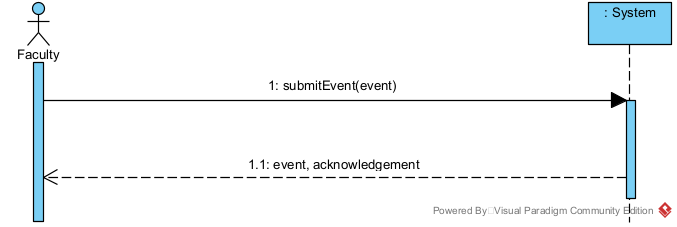
\includegraphics[width=0.8\textwidth]{images/SSD-UC04-CreateEvent.png}
    \centering
    \caption{System Sequence Diagram: Create Event}
\end{figure}

\textbf{Operation:} submitEvent(event: Event) \\
\textbf{Cross References:} UC04 (Create Post) \\
\textbf{Preconditions:}
\begin{itemize}
    \item Faculty, f, has been identified and authenticated.
\end{itemize}
\textbf{Postconditions:}
\begin{itemize}
    \item Event, e, was created.
    \item Event e.status was set to “proposed”.
    \item Event, e, was persisted.
\end{itemize}
%%%%%%%%%%%%%%%%%%%%%%%%%%%%%%%%%%%%%%%%%%%%%%%%%%%%%%%%%%%%%%%%%%%%%%%%%%%%%%%
\subsubsection{UC05: Edit Event}
\textbf{ID:} UC05 (Edit Event) \\
\textbf{Scope:} CS Automated Information Timeline \\
\textbf{Level:} User Goal \\
\textbf{Primary Actor:} Faculty \\
\textbf{Stakeholders and Interests:}
\begin{itemize}
    \item Audience: Wants to view up-to-date information about events in the CS Department
    \item Faculty: Wants the ability to provide updated information on events they submitted
    \item Office Manager: Wants to display accurate event information on the calendar on the Lobby TV
    \item Admin/Reviewer: Wants to update previously approved events with up-to-date information provided by the Faculty who submitted those events
\end{itemize}
\textbf{Preconditions:} Faculty created an event (UC04) and submitted it for review (UC08). Admin/Reviewer reviewed the event (UC09) and approved. Admin/Reviewer is identified and authenticated in the system. Faculty is identified and authenticated in the system and is viewing the event calendar (UC03). \\
\textbf{Postconditions:} Event status is in a proposed state. \\
\textbf{Main Success Scenario:}
\begin{enumerate}
    \item Faculty clicks the ``View My Events'' link on the event calendar page.
    \item System returns a list of existing events authored by Faculty that have been approved.
    \item Faculty selects the event they wish to edit from the returned list of their previously approved events.
    \item System returns the event page for the selected event.
    \item Faculty clicks the “Edit This Event” button on the event page.
    \item Faculty enters the updated event information into the submission form:
          \begin{itemize}
              \item Event date
              \item Event time
              \item Event description
          \end{itemize}
    \item Faculty submits the updated event information for Admin/Reviewer review.
    \item System provides Faculty with a submission confirmation message.
\end{enumerate}
\textbf{Extensions (or Alternate Flows):} \\
3-4a. Faculty begins editing the event, then decides not to submit the updates for review:
\begin{enumerate}
    \item Upon leaving the web page, any changes to event date, time, or description entered into the submission form are erased.
    \item Selected event remains unchanged in the system.
\end{enumerate}
3b. Faculty does not see the event they wish to edit in the returned list because the event has not yet been approved by the Admin/Reviewer:
\begin{enumerate}
    \item Faculty must wait for approval from Admin/Reviewer on the original event before the event is eligible for editing.
\end{enumerate}
\textbf{Special Requirements:} None \\
\textbf{Technology and Data Variations List:} \\
4a. Date input is required in the format MM/DD/YYYY. \\
4b. Time input is required in the Standard Time format in the Central Time Zone. \\
\textbf{Frequency of Occurrence:} Could be nearly continuous if Admin/Reviewer also reviews edited events and approves them (UC09) nearly continuously. \\
\textbf{Open Issues:} None \\

\begin{figure}[H]
    \centering
    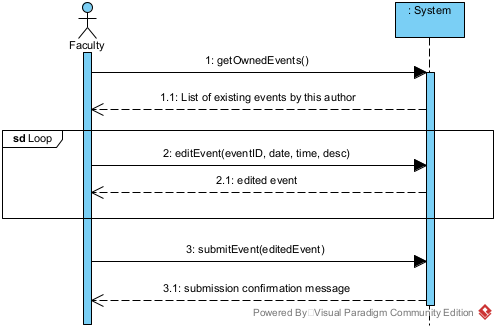
\includegraphics[width=0.8\textwidth]{images/SSD-UC05-EditEvent.png}
    \centering
    \caption{System Sequence Diagram: Edit Event}
\end{figure}

\textbf{Operation:} getOwnedEvents() \\
\textbf{Cross-References:} UC05 (Edit Event), UC06 (Delete Event), UC07 (View Event) \\
\textbf{Pre-conditions:} Event object has been created. Event has been associated with Faculty. Event attribute status is set to approved. \\
\textbf{Post-conditions:} None. \\

\textbf{Operation:} editEvent(eventID, date, time, desc) \\
\textbf{Cross-References:} UC05 (Edit Event) \\
\textbf{Pre-conditions:}
\begin{itemize}
    \item Event object has been created.
    \item Event attribute status is set to approved.
    \item Event has been associated with Faculty.
\end{itemize}
\textbf{Post-conditions:} editedEvent has been created.
\begin{itemize}
    \item editedEvent object has been created.
    \item editedEvent attributes (date, time, desc) have been updated.
    \item editedEvent has been associated with Faculty.
\end{itemize}

\textbf{Operation:} submitEvent(editedEvent) \\
\textbf{Cross-References:} UC05 (Edit Event) \\
\textbf{Pre-conditions:}
\begin{itemize}
    \item editedEvent object has been created.
    \item editedEvent attributes (date, time, desc) have been updated.
    \item editedEvent has been associated with Faculty.
\end{itemize}
\textbf{Post-conditions:}
\begin{itemize}
    \item Notification object is created.
    \item Notification object is associated with editedEvent, Faculty, and Admin/Reviewer.
\end{itemize}
%%%%%%%%%%%%%%%%%%%%%%%%%%%%%%%%%%%%%%%%%%%%%%%%%%%%%%%%%%%%%%%%%%%%%%%%%%%%%%%
\subsubsection{UC06: Delete Event}
\textbf{ID:} UC06 (Delete Event) \\
\textbf{Scope:} CS Automated Information Timeline \\
\textbf{Level:} user goal \\
\textbf{Stakeholders and Interests:}
\begin{itemize}
    \item Audience: Wants to view up-to-date information about events in the CS Department
    \item Faculty: Wants the ability to delete events that they submitted that are no longer happening
    \item Office Manager: Wants to display accurate event information on the calendar on the Lobby TV
\end{itemize}
\textbf{Preconditions:} Faculty created an event (UC04) and submitted it for review (UC08). Admin/Reviewer reviewed the event (UC09) and approved. Faculty is identified and authenticated in the system and is viewing the event calendar (UC03). \\
\textbf{Postconditions:} Event status is in a deleted state. \\
\textbf{Main Success Scenario:}
\begin{enumerate}
    \item Faculty clicks the ``View My Events'' link on the event calendar page.
    \item System returns a list of existing events authored by Faculty that have been approved.
    \item Faculty selects the event they wish to delete from the returned list of their previously approved events.
    \item System returns the event page for the selected event.
    \item Faculty clicks the ``Delete This Event'' button on the event page.
    \item System prompts Faculty to confirm the removal of the event from the event calendar.
    \item Faculty confirms the removal of the event from the event calendar by clicking ``Yes''.
    \item System provides Faculty with a confirmation message.
\end{enumerate}
\textbf{Extensions (or Alternate Flows):} \\
3a. Faculty does not see the event they wish to delete in the returned list because the event has not yet been approved by the Admin/Reviewer:
\begin{enumerate}
    \item Faculty must wait for approval from Admin/Reviewer on the original event before the event is eligible for removal from the event calendar.
\end{enumerate}
7a. Faculty decides they do not want to remove the event from the event calendar:
\begin{enumerate}
    \item Faculty clicks the ``No'' button and is redirected to the list of existing events authored by Faculty that have been approved.
\end{enumerate}
\textbf{Special Requirements:} None \\
\textbf{Technology and Data Variations List:} None \\
\textbf{Frequency of Occurrence:} Maximum once per submitted and approved event. \\
\textbf{Open Issues:} None \\

\begin{figure}[H]
    \centering
    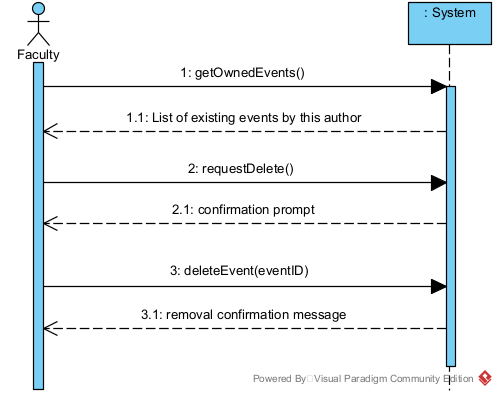
\includegraphics[width=0.8\textwidth]{images/SSD-UC06-DeleteEvent.png}
    \centering
    \caption{System Sequence Diagram: Delete Event}
\end{figure}

\textbf{Operation:} requestDelete() \\
\textbf{Cross-References:} UC06 (Delete Event) \\
\textbf{Pre-conditions:}
\begin{itemize}
    \item Event object has been created.
    \item Event attribute status is set to approved.
    \item Event has been associated with Faculty.
\end{itemize}
\textbf{Post-conditions:} None \\

\textbf{Operation:} deleteEvent(eventID) \\
\textbf{Cross-References:} UC06 (Delete Event) \\
\textbf{Pre-conditions:}
\begin{itemize}
    \item Event object has been created.
    \item Event attribute status is set to approved.
    \item Event has been associated with Faculty.
\end{itemize}
\textbf{Post-conditions:}
\begin{itemize}
    \item Event attribute status is set to deleted.
    \item Event associated with Faculty has been broken.
\end{itemize}
%%%%%%%%%%%%%%%%%%%%%%%%%%%%%%%%%%%%%%%%%%%%%%%%%%%%%%%%%%%%%%%%%%%%%%%%%%%%%%%
\subsubsection{UC07: View Event}
\textbf{ID:} UC07 (View Event) \\
\textbf{Scope:} CS Automated Information Timeline \\
\textbf{Level:} user goal \\
\textbf{Stakeholders and Interests:}
\begin{itemize}
    \item Audience: Wants to view up-to-date information about events in the CS Department
    \item Faculty: Wants the ability to view events they have submitted
    \item Office Manager: Wants to display calendar events on the Lobby TV
    \item Admin/Reviewer: Wants to view events submitted by Faculty so they can review them
\end{itemize}
\textbf{Preconditions:} Faculty created an event (UC04) and submitted it for review (UC08). Admin/Reviewer reviewed the event (UC09) and approved. Faculty is identified and authenticated in the system and is viewing the event calendar (UC03). \\
\textbf{Postconditions:} Event status is in an approved state. \\
\textbf{Main Success Scenario:}
\begin{enumerate}
    \item Faculty clicks the “View My Events” link on the event calendar page.
    \item System returns a list of existing events authored by Faculty that have been approved.
    \item Faculty selects the event they wish to view from the returned list of their previously approved events.
    \item System returns the event page for the selected event.
\end{enumerate}
\textbf{Extensions (or Alternate Flows):} \\
3a. Faculty does not see the event they wish to view in the returned list because the event has not yet been approved by the Admin/Reviewer:
\begin{enumerate}
    \item Faculty must wait for approval from Admin/Reviewer on the original event before the event is eligible for viewing from the event calendar.
\end{enumerate}
\textbf{Special Requirements:} None \\
\textbf{Technology and Data Variations List:} None \\
\textbf{Frequency of Occurrence:} Continuous \\
\textbf{Open Issues:} None \\

\begin{figure}[H]
    \centering
    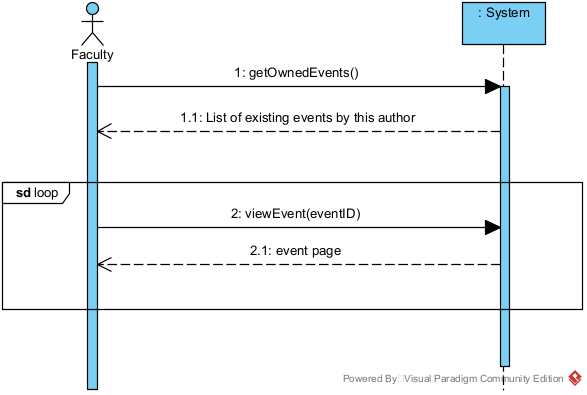
\includegraphics[width=0.8\textwidth]{images/SSD-UC07-ViewEvent.png}
    \centering
    \caption{System Sequence Diagram: View Event}
\end{figure}

\textbf{Operation:} viewEvent(eventID) \\
\textbf{Cross-References:} UC07 (View Event) \\
\textbf{Pre-conditions:}
\begin{itemize}
    \item Event object has been created.
    \item Event attribute status is set to approved.
    \item Event has been associated with Faculty.
\end{itemize}
\textbf{Post-conditions:} None \\
%%%%%%%%%%%%%%%%%%%%%%%%%%%%%%%%%%%%%%%%%%%%%%%%%%%%%%%%%%%%%%%%%%%%%%%%%%%%%%%
\subsubsection{UC08: Submit For Review}
\textbf{Main Success Scenario:} A faculty user submits a post, event, media, or page to the system. The system generates an id and a timestamp that is set to the system time upon submission and associates these attributes with the post, event, media, or page object. The system associates the faculty user that submitted with the post, event, media, or page. The system assigns the status of the post, event, media, or page to the proposed status. The system generates a notification object and attaches the post, event, media, or page object with the notification. The system persists both the created post, event, media, or page object and the created notification object to the database. The created post, event, media, or page is returned to the faculty user. \\
\\
\textbf{Alternative Flows:}
\begin{itemize}
    \item The post, event, media, page, or notification object is not persisted.
    \begin{itemize}
        \item The system will respond to the faculty user with an error message indicating the reason for persistence failure.
        \item The faculty member will correct the identified error and attempt to resubmit the post, event, media, or page item.
    \end{itemize}
    \item If the system does not respond within a given timeframe.
    \begin{itemize}
        \item The system will return an error message to the faculty user indicating a timeout has occurred.
        \item The faculty user will reattempt the submission of the post, event, media, or page item.
        \begin{itemize}
            \item If the system continues to fail to respond within a given timeframe.
            \begin{itemize}
                \item The faculty user will inform the admin/reviewer of the error.
                \item The admin/reviewer will restart the system.
                \item The faculty user will reattempt submission of the post, event, media, or page item.
            \end{itemize}
        \end{itemize}
    \end{itemize}
\end{itemize}

% \begin{figure}[H]
%     \centering
%     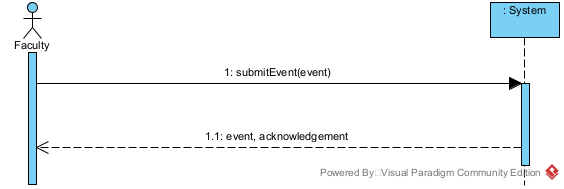
\includegraphics[width=0.8\textwidth]{images/SSD-UC08-SubmitForReview.png}
%     \centering
%     \caption{System Sequence Diagram: Submit For Review}
% \end{figure}
%%%%%%%%%%%%%%%%%%%%%%%%%%%%%%%%%%%%%%%%%%%%%%%%%%%%%%%%%%%%%%%%%%%%%%%%%%%%%%%
\subsubsection{UC09: Review For Approval}
\textbf{ID:} UC09 (Review for Approval) \\
\textbf{Scope:} CS Automated Information Timeline \\
\textbf{Level:} User Goal \\
\textbf{Stakeholders and Interests:}
\begin{itemize}
    \item Faculty: A person that works for the university and is interested in gaining visibility of their post and/or event.
    \item Administrator/Reviewer: A person that works for the university and is interested in reviewing and approving requests for system content additions.
\end{itemize}
\textbf{Preconditions:}
\begin{itemize}
    \item Administrator/Reviewer a has been identified and authenticated.
    \item Notification n has been created and persisted.
    \item n.event, n.post, or n.media has been set.
\end{itemize}
\textbf{Postconditions:}
\begin{itemize}
    \item Notification n.entity was identified as either a Post, Event, or Media.
    \item n.entity.status was set to either “Approved” or “Rejected”.
    \item If the review was favorable, n.entity.status was set to “Approved”.
    \item If the review was unfavorable, n.entity.status was set to “Rejected”.
    \item n.reviewer was set to a.
    \item n.entity was persisted.
\end{itemize}
\textbf{Main Success Scenario:}
\begin{enumerate}
    \item Administrator/Reviewer, a, gets all notifications.
    \item For each Notification, n, in notifications, Administrator/Reviewer, a, performs manual review of the Post, Event, or Media attached to Notification, n.
    \item Administrator/Reviewer, a, updates the Post, Event, or Media that was attached to Notification, n, to either “Approved” or “Rejected”.
    \item If the review is favorable, n.event.status, n.post.status, or n.media.status is set to “Approved”.
    \item If the review is not favorable, n.event.status, n.post.status, or n.media.status is set to “Rejected”.
    \item The system persists the updated Post, Event, or Media with the status set by Administrator/Reviewer, a.
    \item The system associates Administrator/Reviewer, a, with Notification n.
    \item Notification, n, is persisted.
    \item The Event, Post, or Media is persisted.
\end{enumerate}
\textbf{Extensions:} \\
2a. There are multiple objects, Post, Event, or Media, attached to Notification n.
\begin{itemize}
    \item Administrator/Reviewer, a, deletes Notification, n.
\end{itemize}
\textbf{Special Requirements:} None \\
\textbf{Technology and Data Variation List:}
\begin{itemize}
    \item Notification n.post is set and of Post type; n.event and n.media are null.
    \item Notification n.event is set and of Event type; n.post and n.media are null.
    \item Notification n.media is set and of Media type; n.post and n.event are null.
\end{itemize}
\textbf{Frequency of Occurrence:} Could be nearly continuous. \\

\begin{figure}[H]
    \centering
    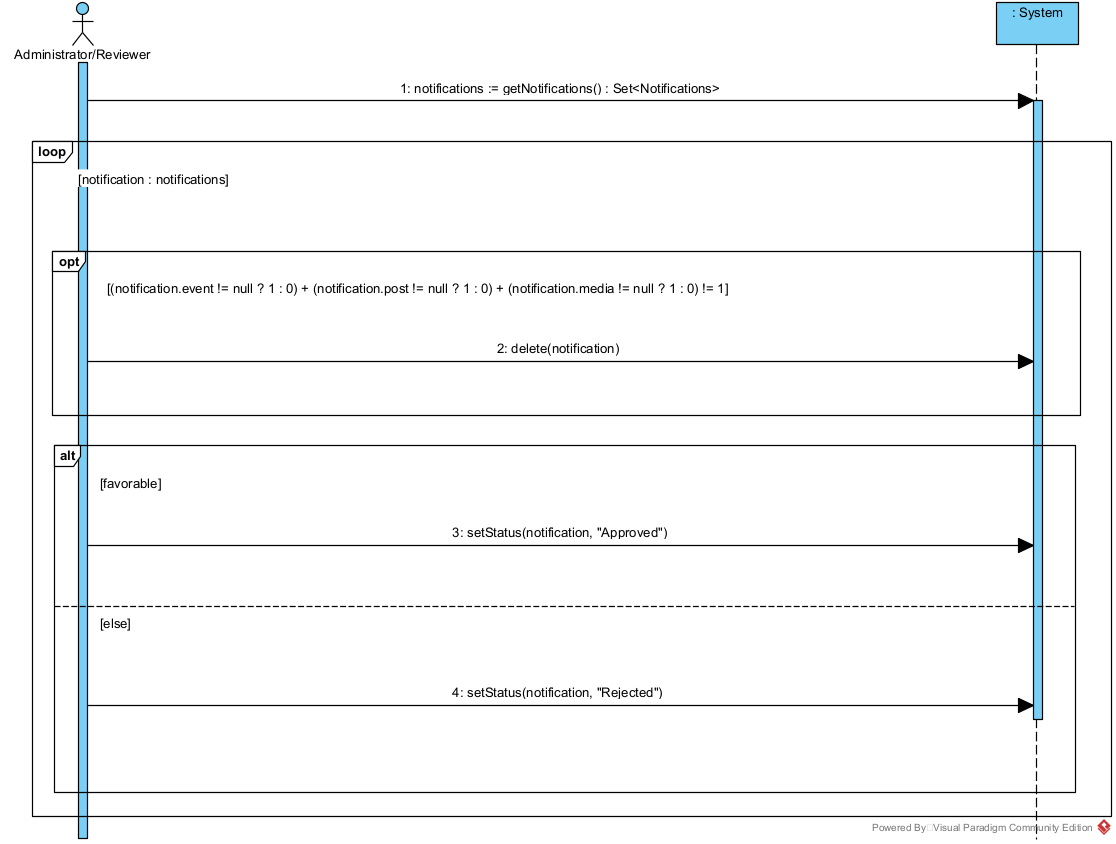
\includegraphics[width=0.8\textwidth]{images/SSD-UC09-ReviewForApproval.png}
    \centering
    \caption{System Sequence Diagram: Review For Approval}
\end{figure}
%%%%%%%%%%%%%%%%%%%%%%%%%%%%%%%%%%%%%%%%%%%%%%%%%%%%%%%%%%%%%%%%%%%%%%%%%%%%%%%
\subsubsection{UC10: Create Post}
\textbf{ID:} UC10 (Create Post) \\
\textbf{Scope:} CS Automated Information Timeline \\
\textbf{Level:} User Goal \\
\textbf{Stakeholders and Interests:}
\begin{itemize}
    \item Faculty: A person who works for the university and is interested in gaining visibility of this post and/or event.
    \item Admin/Reviewer: A person who works for the university and approves and/or removes posts and/or event from the system.
\end{itemize}
\textbf{Preconditions:}
\begin{itemize}
    \item Faculty, f, has been identified and authenticated.
\end{itemize}
\textbf{Postconditions:}
\begin{itemize}
    \item Post, p, was created.
    \item p.status was set to “Pending”.
    \item p.createdBy was set to Faculty f.
    \item Post, p, was persisted.
    \item Notification, n, was created.
    \item n.post was set to Post p.
    \item Notification, n, was persisted.
\end{itemize}
\textbf{Main Success Scenario:}
\begin{enumerate}
    \item Faculty writes the post using the post creation tool.
    \item The post title is written by the faculty user.
    \item The post body is written by the faculty user.
    \item Faculty reviews the post draft.
    \item Faculty submits the post to the system.
    \item A post id is generated by the system.
    \item A timestamp is generated by the system.
    \item The user id of the faculty user is attached to the post object.
    \item The system assigns the status of the post to the proposed state.
    \item The system generates a notification object.
    \item The post object is attached to the notification object.
    \item The post object is persisted.
    \item The notification object is persisted.
    \item The system returns the persisted post object to the faculty user.
\end{enumerate}
\textbf{Extensions:} \\\relax
*.a. Anytime the system does not respond.
\begin{enumerate}
    \item Faculty will notify the Admin/Reviewer.
    \item Admin/Reviewer will restart the system.
    \item Faculty will recreate and submit the post.
\end{enumerate}
5.a. Anytime the system does not respond.
\begin{enumerate}
    \item The system will return an error message to the faculty user.
    \item The faculty user will resubmit the post.
\end{enumerate}
6.a. If the post is not persisted.
\begin{enumerate}
    \item The system will return an error message to the faculty user.
    \item The faculty user will reattempt the submission of the post.
\end{enumerate}
\textbf{Special Requirements:} None \\
\textbf{Technology and Data Variations List: }
\begin{enumerate}
    \item Date will be of the format “yyyy-MM-ddTHH:mm:ss”.
    \item Id will be of the format of a universally unique identifier, UUID.
\end{enumerate}
\textbf{Frequency of Occurrence:} Could be nearly continuous. \\

\begin{figure}[H]
    \centering
    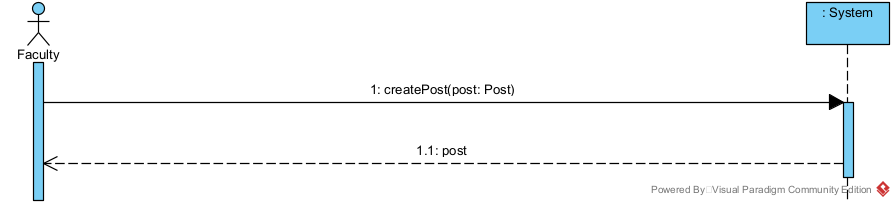
\includegraphics[width=0.8\textwidth]{images/SSD-UC10-CreatePost.png}
    \centering
    \caption{System Sequence Diagram: Edit Post}
\end{figure}
%%%%%%%%%%%%%%%%%%%%%%%%%%%%%%%%%%%%%%%%%%%%%%%%%%%%%%%%%%%%%%%%%%%%%%%%%%%%%%%
\subsubsection{UC11: Edit Post}
\textbf{ID:} UC11 (Edit Post) \\
\textbf{Scope:} CS Automated Information Timeline \\
\textbf{Level:} User goal \\
\textbf{Primary Actor:} Faculty or Admin/Reviewer \\
\textbf{Stakeholders and Interests:}
\begin{itemize}
    \item Audience: A person that is interested in viewing all approved content on the system using their mobile device.
    \item Faculty: A person that works for the university and is interested in gaining visibility of their post and/or event.
    \item Office Manager: A person that works for the university and is interested in prioritizing the order of posts and/or events.
    \item Admin/Reviewer: A person that works for the university and approves and/or removes posts and/or events from the system.
\end{itemize}
\textbf{Preconditions:}
\begin{itemize}
    \item Faculty has been identified and authenticated.
    \item A post has been created.
\end{itemize}
\textbf{Postconditions:}
\begin{itemize}
    \item Post has been updated and saved to database.
    \item Media library has been updated with new images and videos from the updated post.
    \item The display board reflects the updated post flagged for display.
\end{itemize}
\textbf{Main Success Scenario:}
\begin{enumerate}
    \item User selects a post to edit
    \item System opens the editable view for the selected post with options to edit the text, delete the photos and videos, if present, on the post, upload photos and videos on the post and update the display flag.
    \item User saves the updated post.
    \item System presents the confirmation that the post is updated
\end{enumerate}
\textbf{Alternative Flows:}  \\
a. At any time, system fails or becomes unresponsive and does not provide an error message
\begin{enumerate}
    \item User performs a hard refresh on the browser (ctrl + f5 or shift + reload)
    \item System reloads the editable view for the post
\end{enumerate}
b. (3.a) Uploaded media is in unsupported format or exceeds the file size limit
\begin{enumerate}
    \item System prompts the user with the appropriate error message
    \item User acknowledges the error and reuploads the media in supported format and size.
\end{enumerate}

\begin{figure}[H]
    \centering
    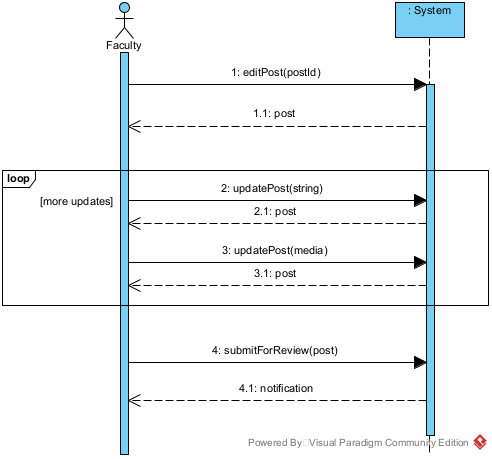
\includegraphics[width=0.8\textwidth]{images/SSD-UC11-EditPost.png}
    \centering
    \caption{System Sequence Diagram: Edit Post}
\end{figure}

\textbf{Operation:} updatePost(post) \\
\textbf{Cross Reference:} UC11 (Edit Post) \\
\textbf{Preconditions: }
\begin{itemize}
    \item Faculty has been identified and authenticated.
    \item A post has been created and persisted in the database.
    \item Update operation is underway.
\end{itemize}
\textbf{Postconditions:}
\begin{itemize}
    \item A Post instance, post was created
    \item post was associated with the Update operation.
    \item post was modified
    \item Modified post was persisted to the database
\end{itemize}
%%%%%%%%%%%%%%%%%%%%%%%%%%%%%%%%%%%%%%%%%%%%%%%%%%%%%%%%%%%%%%%%%%%%%%%%%%%%%%%
\subsubsection{UC12: Delete Post}
\textbf{ID:} UC12 (Delete Post) \\
\textbf{Scope:} CS Automated Information Timeline \\
\textbf{Level:} User goal \\
\textbf{Primary Actor:} Faculty or Admin/Reviewer \\
\textbf{Stakeholders and Interests: }
\begin{itemize}
    \item Audience: A person that is interested in viewing all approved content on the system using their mobile device.
    \item Faculty: A person that works for the university and is interested in gaining visibility of their post and/or event.
    \item Office Manager: A person that works for the university and is interested in prioritizing the order of posts and/or events.
    \item Admin/Reviewer: A person that works for the university and approves and/or removes posts and/or events from the system.
\end{itemize}
\textbf{Preconditions:}
\begin{itemize}
    \item Faculty has been identified and authenticated.
    \item A post to be deleted exists.
\end{itemize}
\textbf{Postconditions:}
\begin{itemize}
    \item The post has been deleted from the database.
    \item Media library has been updated.
    \item The display board no longer displays the deleted post.
\end{itemize}
\textbf{Main Success Scenario: }
\begin{enumerate}
    \item User navigates to the admin dashboard and accesses the manage post view.
    \item User selects the post to be managed and clicks the delete post button.
    \item System presents the confirmation window prompting the user if they are sure about deleting the post
    \item User confirms deletion.
    \item The system deletes the selected post from the database and updates the display board contents.
    \item System presents the confirmation that the post is deleted
\end{enumerate}
\textbf{Alternative Flows: } \\
a. At any time, system fails or becomes unresponsive and does not provide an error message
\begin{enumerate}
    \item User performs a hard refresh on the browser (ctrl + f5 or shift + reload)
    \item System reloads the editable view for the post
\end{enumerate}
b. (4.a) User does not confirm post deletion (clicks no)
\begin{enumerate}
    \item No action is taken, and the post is displayed in manage post view
\end{enumerate}

\begin{figure}[H]
    \centering
    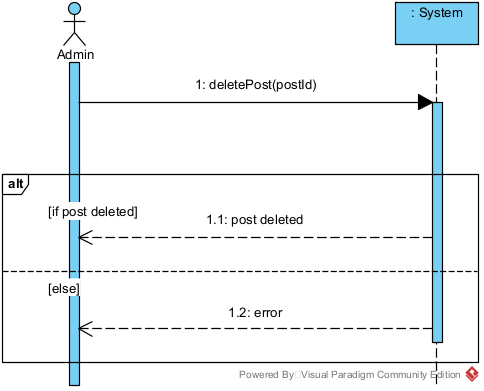
\includegraphics[width=0.8\textwidth]{images/SSD-UC12-DeletePost.png}
    \centering
    \caption{System Sequence Diagram: Delete Post}
\end{figure}

\textbf{Operation:} deletePost(postId) \\
\textbf{Cross Reference:} UC12  (Delete Post) \\
\textbf{Preconditions:}
\begin{itemize}
    \item Faculty has been identified and authenticated.
    \item A post has been created and persisted in the database.
    \item Delete operation is underway.
\end{itemize}
\textbf{Postconditions:}
\begin{itemize}
    \item A Post instance, post was created
    \item post was associated with the Delete operation.
    \item post was deleted
\end{itemize}
%%%%%%%%%%%%%%%%%%%%%%%%%%%%%%%%%%%%%%%%%%%%%%%%%%%%%%%%%%%%%%%%%%%%%%%%%%%%%%%
\subsubsection{UC13: View Post}
\textbf{ID:} UC13 (View Post) \\
\textbf{Scope:} CS Automated Information Timeline \\
\textbf{Level:} User goal \\
\textbf{Primary Actor:} Audience \\
\textbf{Stakeholders and Interests: }
\begin{itemize}
    \item Audience: A person that is interested in viewing all approved content on the system using their mobile device.
    \item Faculty: A person that works for the university and is interested in gaining visibility of their post and/or event.
    \item Office Manager: A person that works for the university and is interested in prioritizing the order of posts and/or events.
    \item Admin/Reviewer: A person that works for the university and approves and/or removes posts and/or events from the system.
\end{itemize}
\textbf{Preconditions: }
\begin{itemize}
    \item A post has been created and staged for display.
\end{itemize}
\textbf{Postconditions:} None \\
\textbf{Main Success Scenario: }
\begin{enumerate}
    \item User accesses the web application UI by scanning the QR code on the display board.
    \item System presents the web view with posts staged for display
\end{enumerate}
\textbf{Alternative Flows: } \\
a. At any time, system fails or becomes unresponsive and does not provide an error message
\begin{enumerate}
    \item User performs a hard refresh on the browser (ctrl + f5 or shift + reload)
    \item System reloads the editable view for the post
\end{enumerate}

\begin{figure}[H]
    \centering
    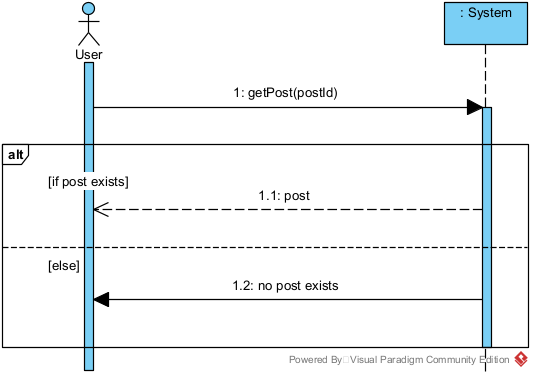
\includegraphics[width=0.8\textwidth]{images/SSD-UC13-ViewPost.png}
    \centering
    \caption{System Sequence Diagram: View Post}
\end{figure}

\textbf{Operation:} getPost(postId) \\
\textbf{Cross Reference:} UC13 (View Post)
\textbf{Preconditions:}
\begin{itemize}
    \item Post exists and is staged for display
    \item User is attempting to view a specific post (request)
\end{itemize}
\textbf{Postconditions:}
\begin{itemize}
    \item A PostService instance, postService  was created
    \item A PostRepository instance postRepository was created
    \item A Post instance post was created
    \item post was associated with the request
\end{itemize}
%%%%%%%%%%%%%%%%%%%%%%%%%%%%%%%%%%%%%%%%%%%%%%%%%%%%%%%%%%%%%%%%%%%%%%%%%%%%%%%
\subsubsection{UC14: Edit Page of Event}
\textbf{ID:} UC14 (Edit Page of Event) \\
\textbf{Precondition:} Office Manager has been identified and authenticated. \\
\textbf{Main Success Scenario:} Office Manager can edit HTML page of the event using the WYSIWYG (What You See Is What You Get) editor. Office Manager can select an event and click the edit option, which will allow them to use the WYSISYG editor to compose and submit the HTML page associated with the event. The changes will take effect immediately and will be reflected on the display board. \\
%%%%%%%%%%%%%%%%%%%%%%%%%%%%%%%%%%%%%%%%%%%%%%%%%%%%%%%%%%%%%%%%%%%%%%%%%%%%%%%
\subsubsection{UC15: Manage Displayed Posts}
\begin{figure}[H]
    \centering
    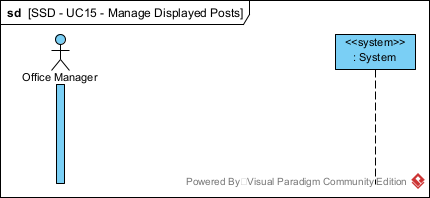
\includegraphics[width=0.8\textwidth]{images/SSD-UC15-ManageDisplayedPosts.png}
    \centering
    \caption{System Sequence Diagram: Manage Displayed Posts}
\end{figure}
%%%%%%%%%%%%%%%%%%%%%%%%%%%%%%%%%%%%%%%%%%%%%%%%%%%%%%%%%%%%%%%%%%%%%%%%%%%%%%%
\subsubsection{UC16: Manage Displayed Media}
\textbf{ID:} UC16 (Manage Media For Display) \\
\textbf{Scope:} CS Automated Information Timeline \\
\textbf{Level:} User goal \\
\textbf{Primary Actor:} Office Manager \\
\textbf{Stakeholders and Interests:}
\begin{itemize}
    \item Admin/Reviewer: Wants to ensure curated list of media items are on display for guests
    \item Guest: Wants to be able to see images and/or video on the TV display
    \item Faculty: Wants to ensure relevant media can be shown to guests.
\end{itemize}
\textbf{Preconditions:}
\begin{itemize}
    \item User with Office Manager role has been authenticated.
    \item Media library is available.
\end{itemize}
\textbf{Postconditions:}
\begin{itemize}
    \item Media is displayed on the TV display
    \item The ordering of the media displayed is correct
\end{itemize}
\textbf{Main Success Scenario:}
\begin{enumerate}
    \item User navigates to media library
    \item The system displays the media library and available files for display
    \item User selects media to be displayed on the main display
    \item The system displays the list of media that will be displayed on the main display
    \item Repeat step 3 and 4 until all required media is selected for display
    \item User reviews final list of media to be displayed
    \item User approves media display and saves new list of media to be displayed
    \item The system records the final list and the user identification associated with the created list
    \item The system updates the main display with the list of media to display
    \item The system provides local copies of media to the main display
    \item The main display begins displaying the listed media
    \item The system notifies the user that the listed media has been saved and is displayed on the main display
\end{enumerate}
\textbf{Alternative Flows:} \\
3A: User does not find suitable media for display and has media to upload
\begin{enumerate}
    \item User selects media they wish to upload from local device
    \item User uploads new media to media library
    \item The system confirms successful upload of media
    \item The system adds newly uploaded media to list of media to display
    \item Proceed to step 4 of the main scenario
\end{enumerate}
3B: User wants to remove items from current Media list
\begin{enumerate}
    \item User proceeds to modify currently returned media list
    \item System returns the current list of media marked for display on the main display
    \item User updates list to remove media
    \item System returns updated list
    \item Repeat step 3 and 4 until either all media is removed from the list or user cancels the action.
    \item Proceed to step 6 of the main scenario
\end{enumerate}
7A: User needs to modify order of media to be displayed
\begin{enumerate}
    \item User selects option to change media ordering
    \item The system notifies the user the current order of media will be lost
    \item User confirms
    \item The system returns user to step 3 of the main scenario
\end{enumerate}

\begin{figure}[H]
    \centering
    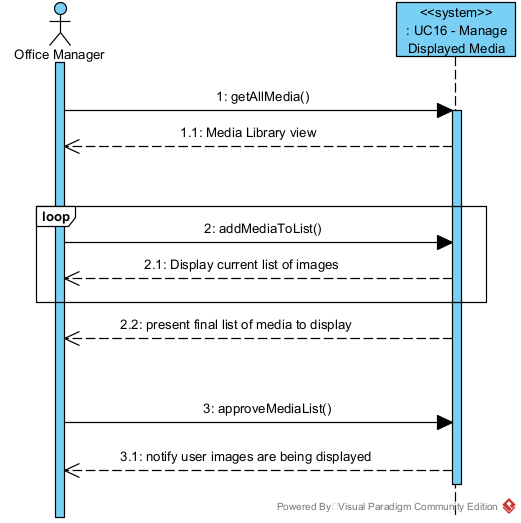
\includegraphics[width=0.8\textwidth]{images/SSD-UC16-ManageDisplayedMedia.png}
    \centering
    \caption{System Sequence Diagram: Manage Displayed Media}
\end{figure}

\textbf{Operation:} getAllMedia() \\
\textbf{Cross-References:} UC16 (Manage Media For Display) \\
\textbf{Pre-conditions:}
\begin{itemize}
    \item Media objects exist in the media library (database store)
    \item Media objects have been approved by admin
\end{itemize}
\textbf{Post-conditions:}
\begin{itemize}
    \item List of media returned to user as List<> object, \emph{ml}
\end{itemize}

\textbf{Operation:} addMediaToList() \\
\textbf{Cross-References:} UC16 (Manage Media For Display) \\
\textbf{Pre-conditions:}
\begin{itemize}
    \item Media List object, \emph{ml}, is not at capacity yet
    \item \emph{ml} has not been approved
\end{itemize}
\textbf{Post-conditions:}
\begin{itemize}
    \item \emph{ml} has association with media item, \emph{m}, formed
    \item \emph{ml} has been updated and requests approval
\end{itemize}

\textbf{Operation:} approveMediaList () \\
\textbf{Cross-References:} UC16 (Manage Media For Display) \\
\textbf{Pre-conditions:}
\begin{itemize}
    \item User has marked \emph{ml} as ready for publish
    \item \emph{ml} is not over capactiy
    \item \emph{ml}  has not been approved yet
\end{itemize}
\textbf{Post-conditions:}
\begin{itemize}
    \item \emph{ml} is approved and set for display
    \item \emph{MainDisplay} updates with new list, \emph{ml}
\end{itemize}

%%%%%%%%%%%%%%%%%%%%%%%%%%%%%%%%%%%%%%%%%%%%%%%%%%%%%%%%%%%%%%%%%%%%%%%%%%%%%%%
\section{Activity Diagram: Create Event}
\begin{figure}[H]
    \centering
    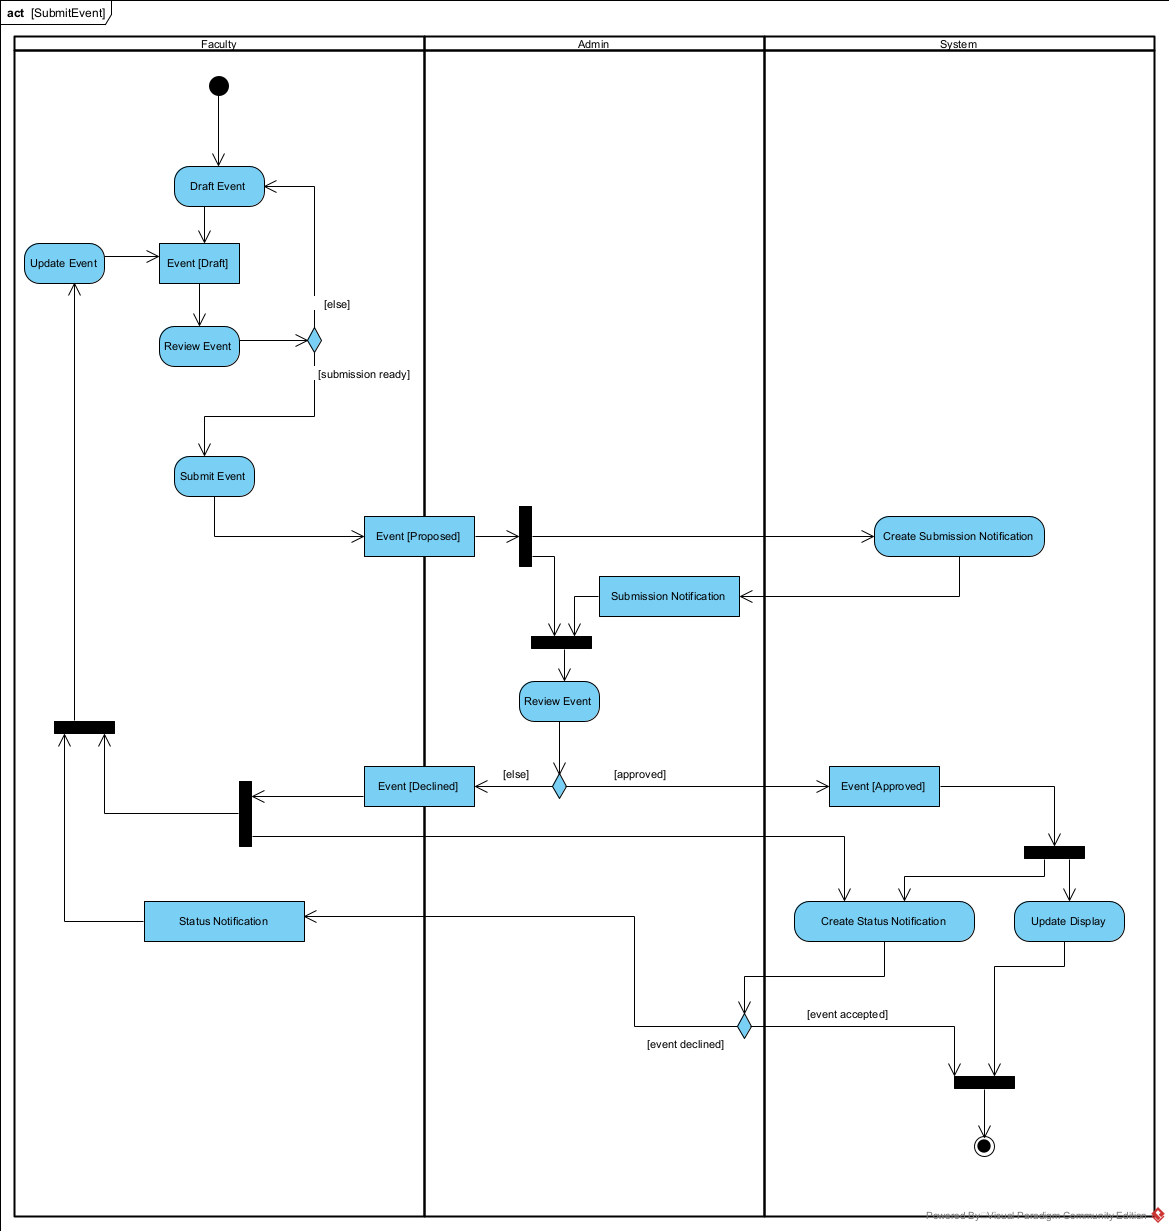
\includegraphics[width=.98\textwidth]{images/SubmitEvent.png}
    \centering
    \caption{Activity Diagram: Create Event}
    \label{fig:activityDiagram}
\end{figure}
%%%%%%%%%%%%%%%%%%%%%%%%%%%%%%%%%%%%%%%%%%%%%%%%%%%%%%%%%%%%%%%%%%%%%%%%%%%%%%%
\section{Wireframes}
\subsection{Faculty Dashboard}
\begin{figure}[H]
    \centering
    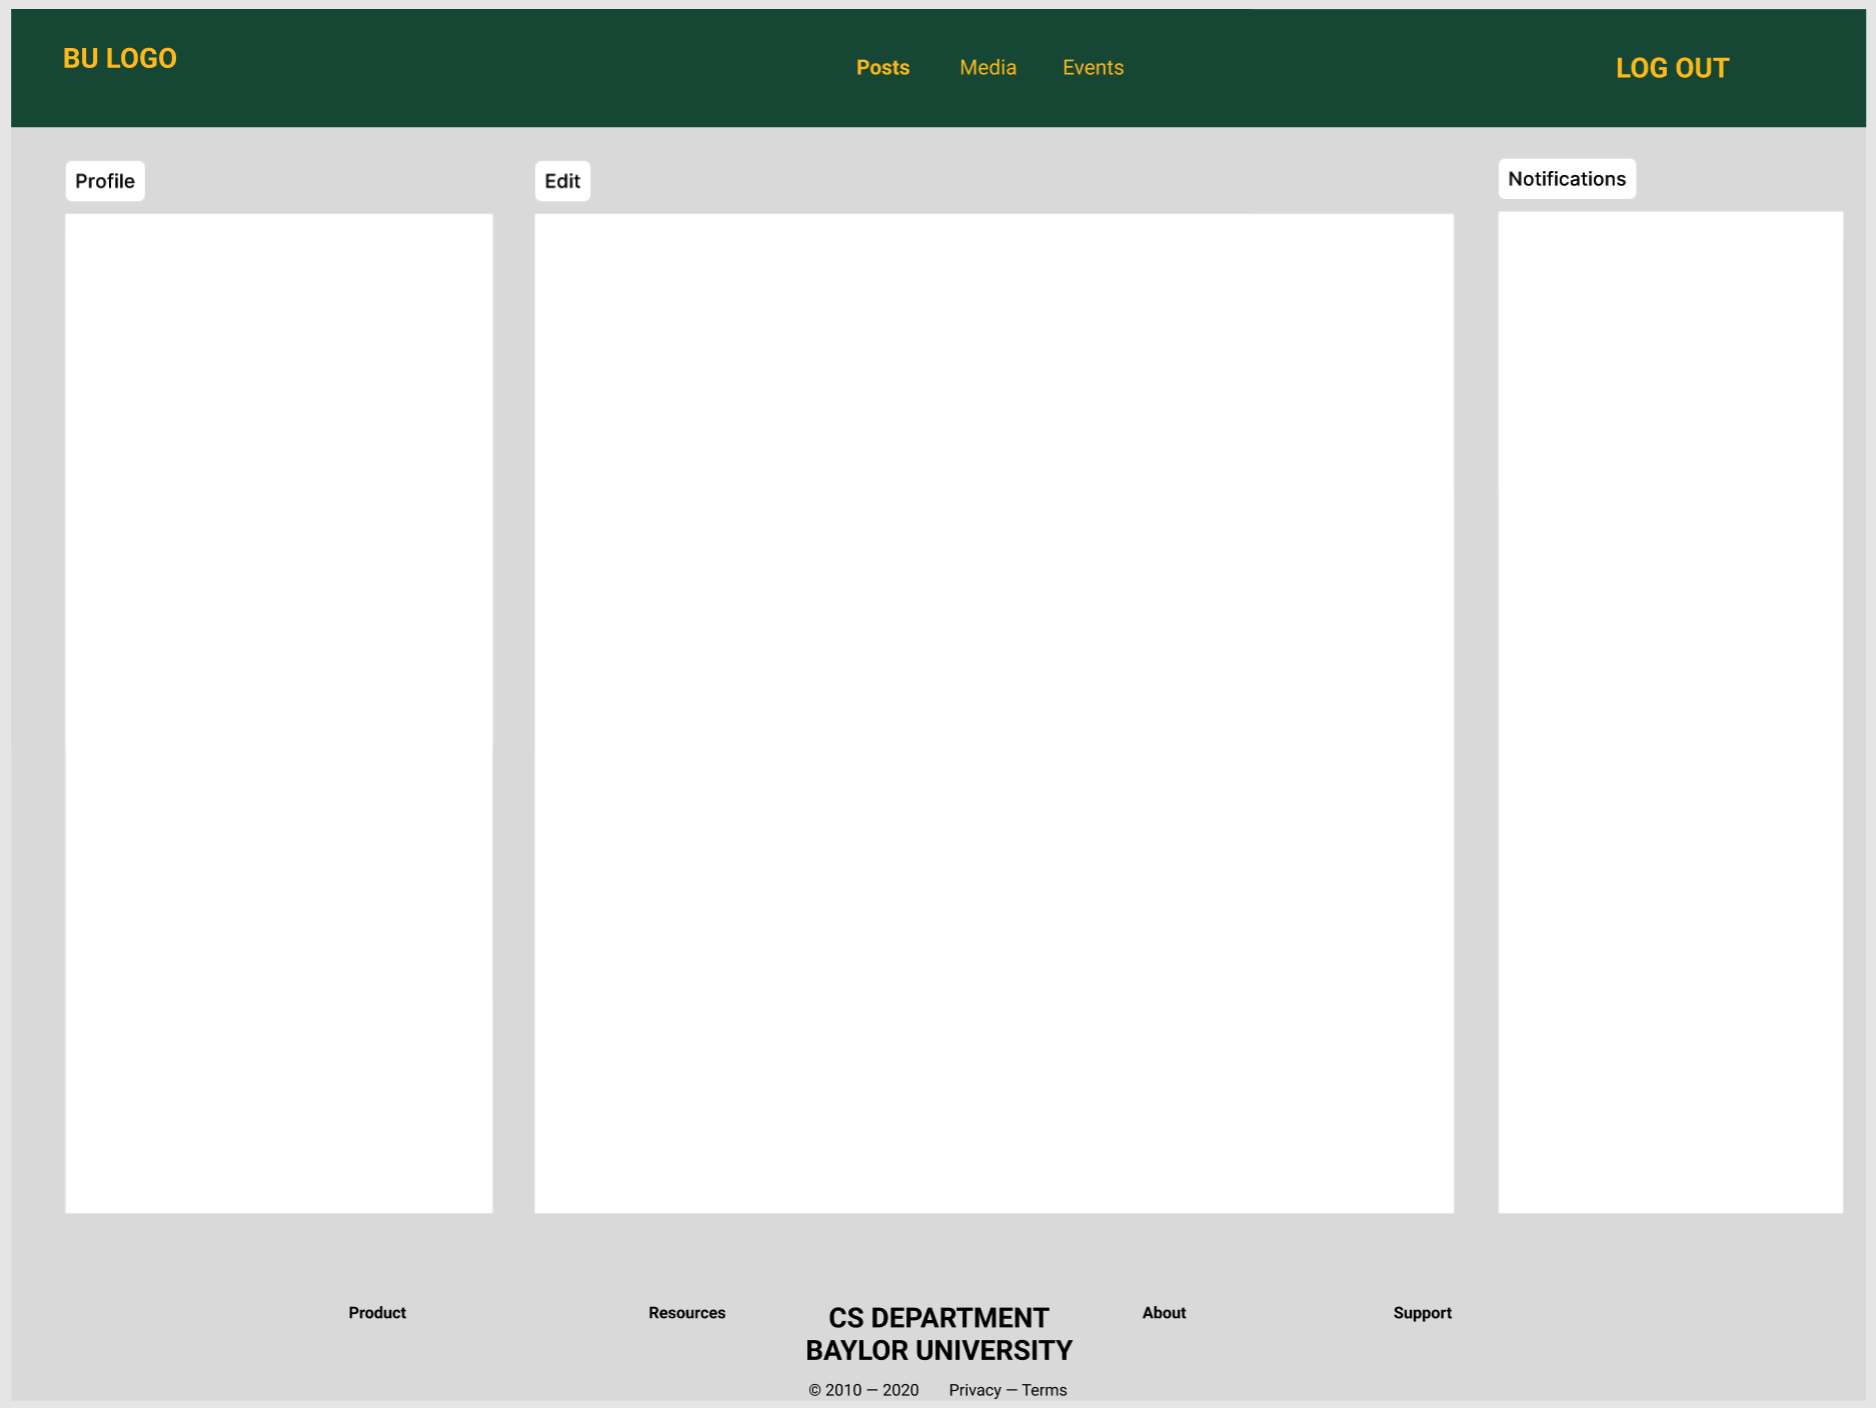
\includegraphics[width=0.8\textwidth]{images/wireframe_FacultyDashboard.png}
    \centering
    \caption{Wireframe: Faculty Dashboard}
\end{figure}

\subsection{TV}
\begin{figure}[H]
    \centering
    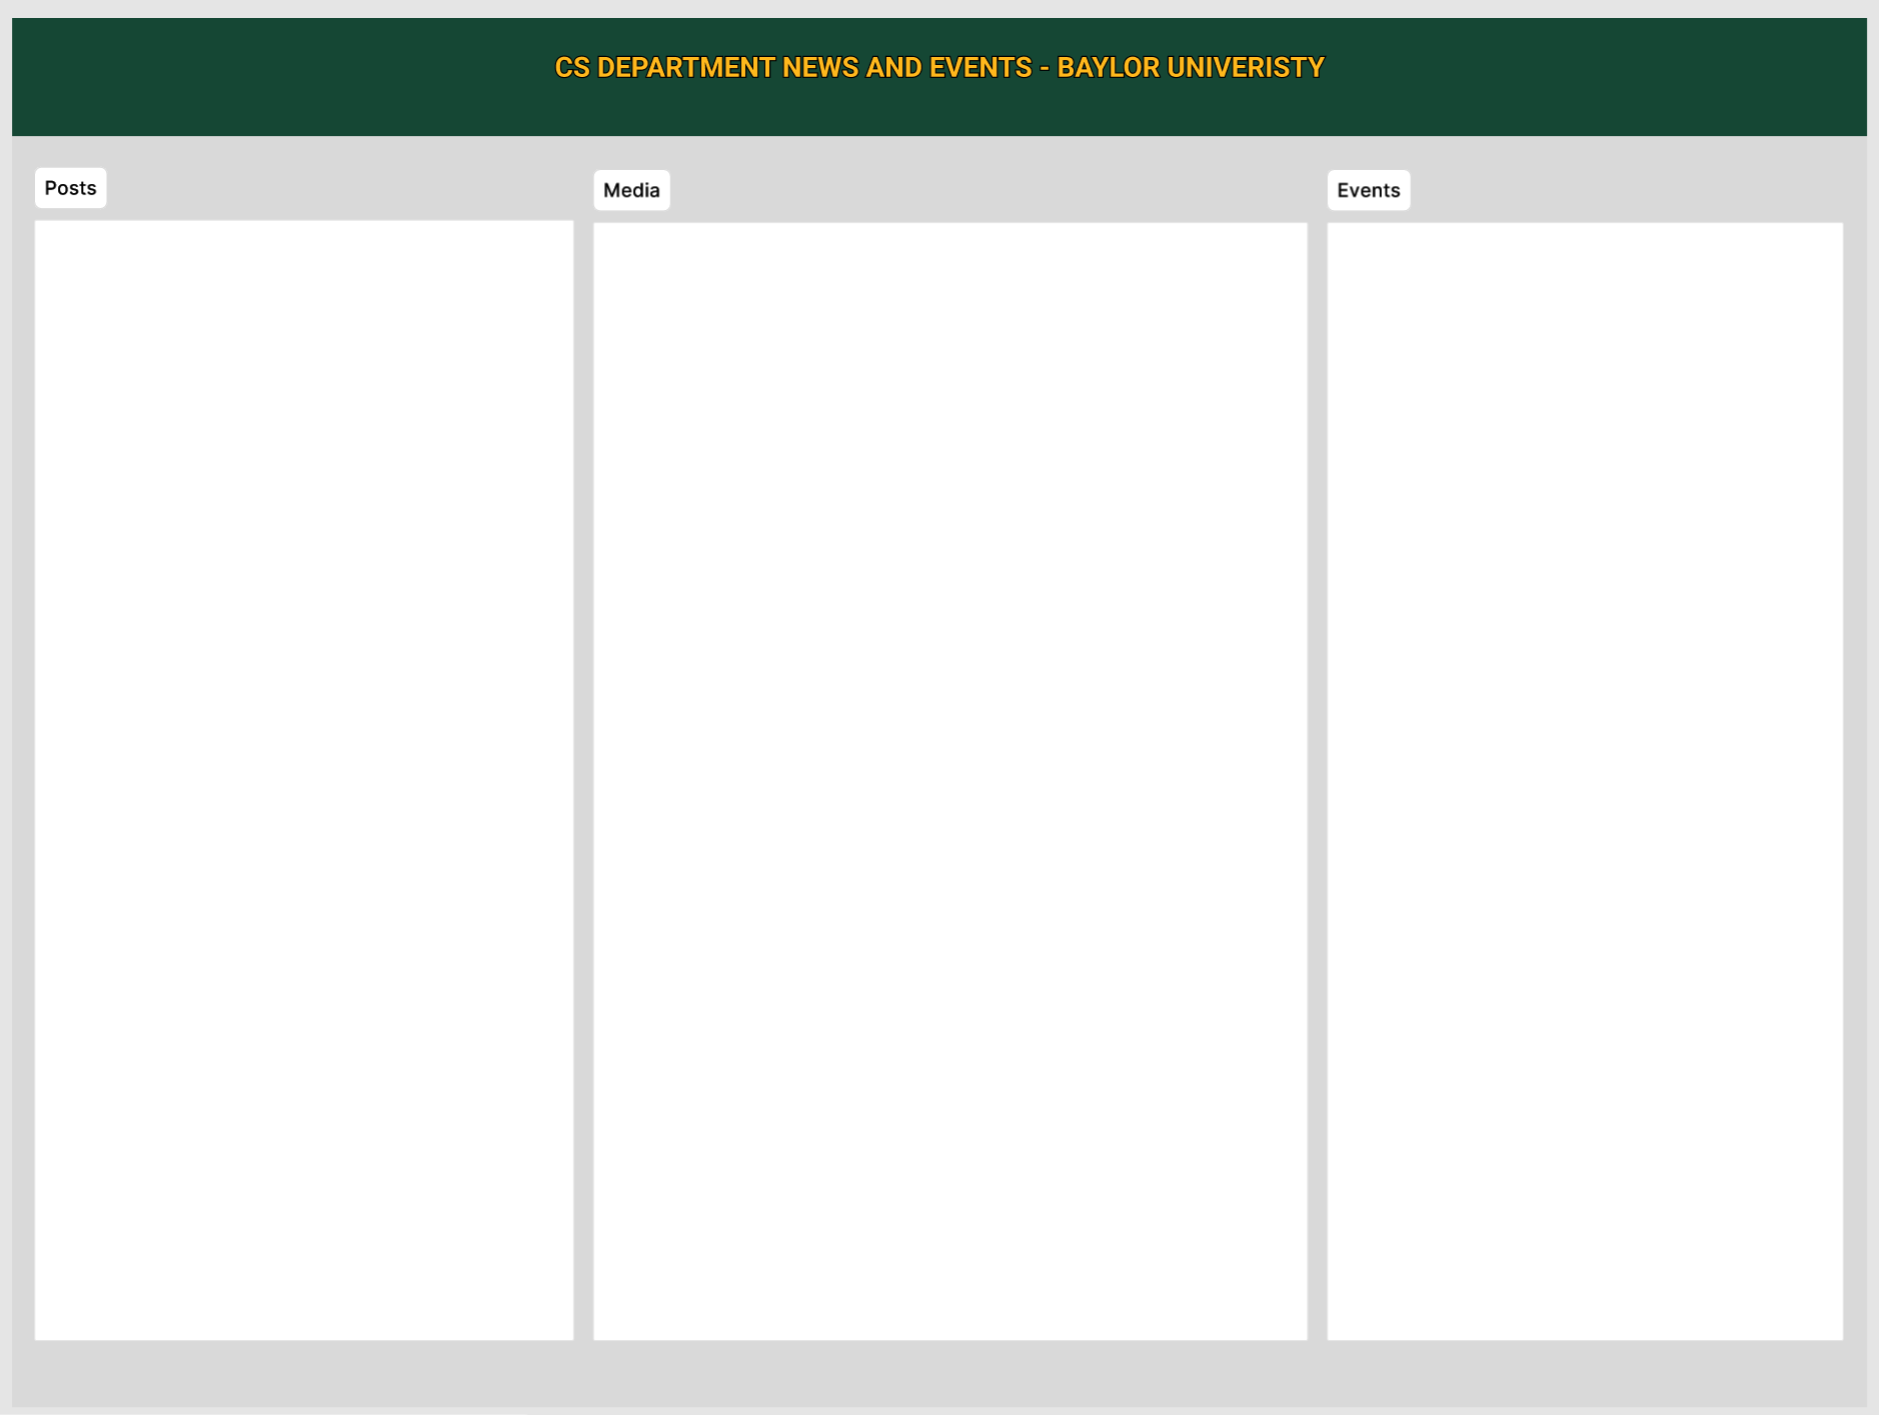
\includegraphics[width=0.8\textwidth]{images/wireframe_TV_Display.png}
    \centering
    \caption{Wireframe: TV}
\end{figure}

\subsection{Web UI}
\begin{figure}[H]
    \centering
    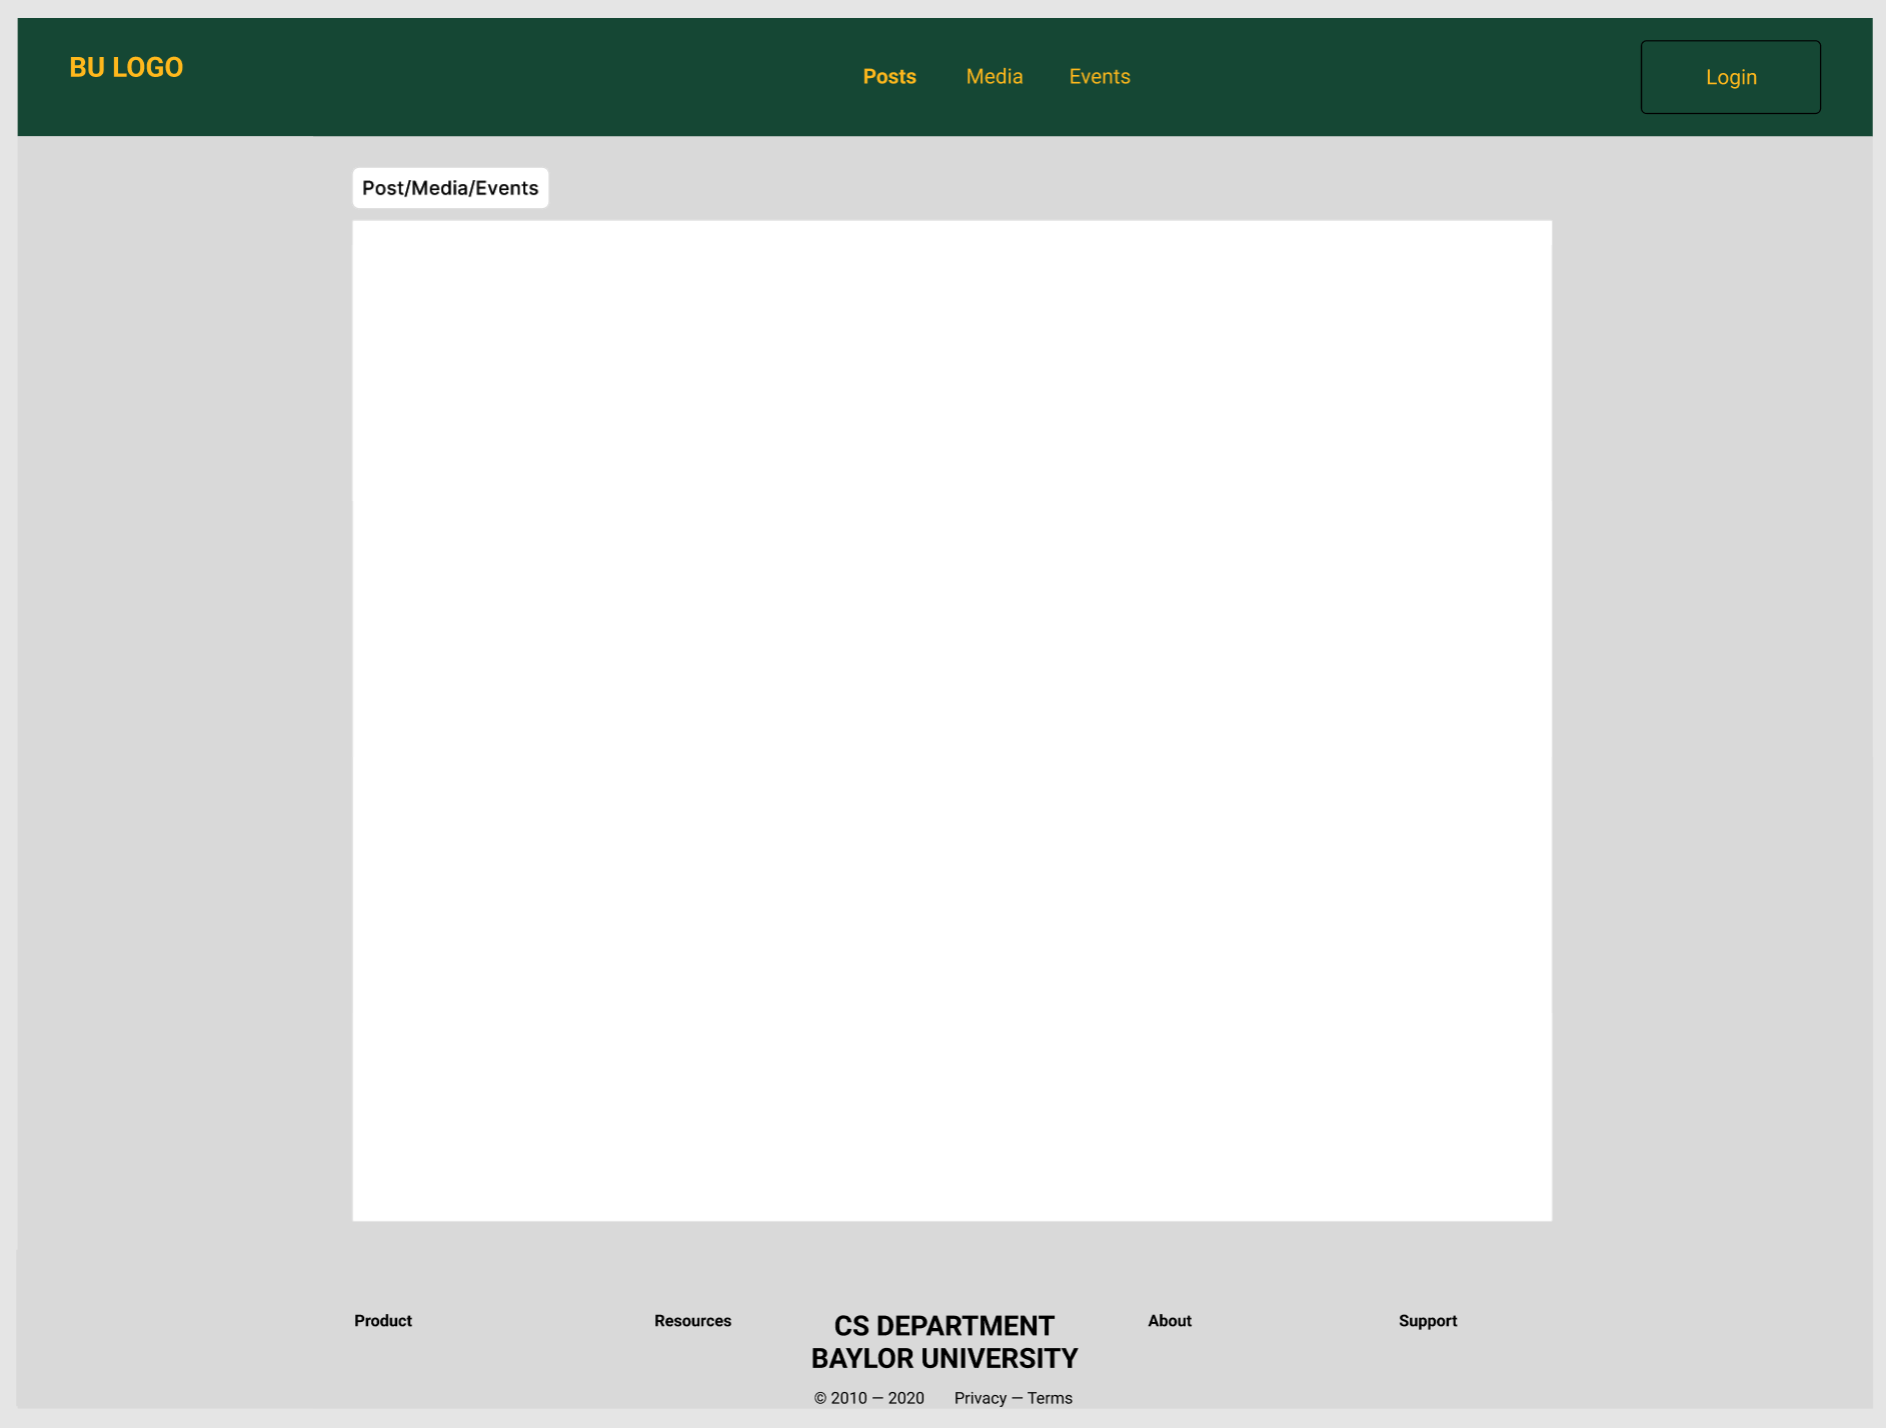
\includegraphics[width=0.8\textwidth]{images/wireframe_webUI.png}
    \centering
    \caption{Wireframe: Web UI}
\end{figure}
%%%%%%%%%%%%%%%%%%%%%%%%%%%%%%%%%%%%%%%%%%%%%%%%%%%%%%%%%%%%%%%%%%%%%%%%%%%%%%%
\section{Class Diagram}
\begin{figure}[H]
    \centering
    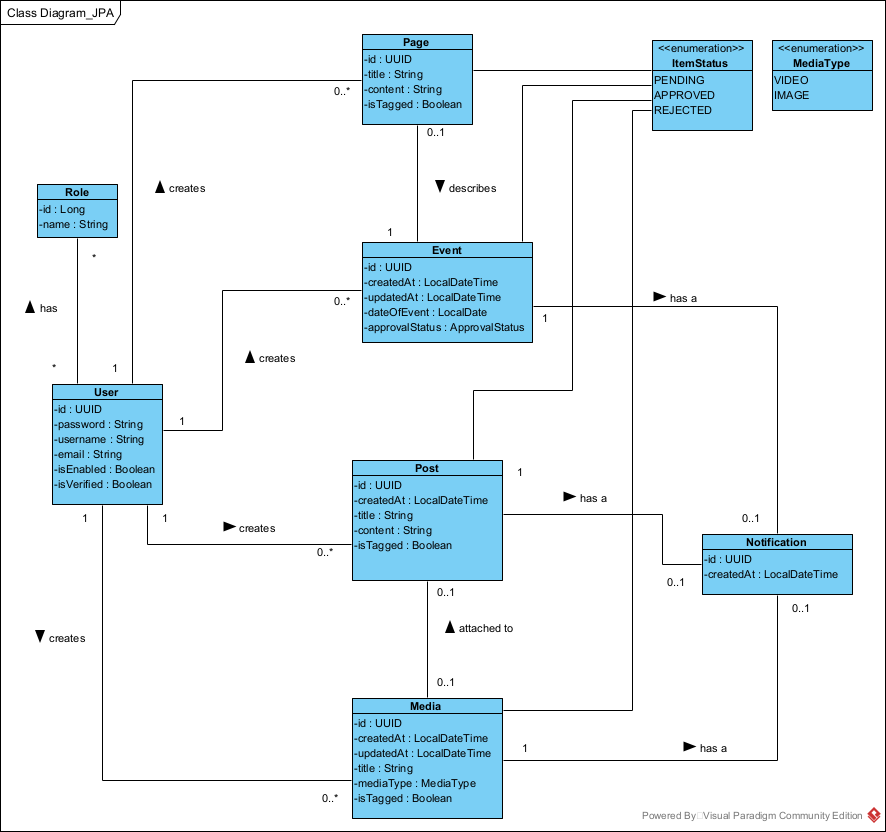
\includegraphics[width=.98\textwidth]{images/ClassDiagram.png}
    \centering
    \caption{Class Diagram}
\end{figure}%%%%%%%%%%%%%%%%%%%%%%%%%%%%%%%%%%%%%%%%%%%%%%%%%%%%%%%%%%%%%%%%%%%%%%%%%%%%%%%
\section{Code}
Note about the code.

\end{document}